\begin{frame}{The models work, and they separate by difficulty as designed}
\begin{center}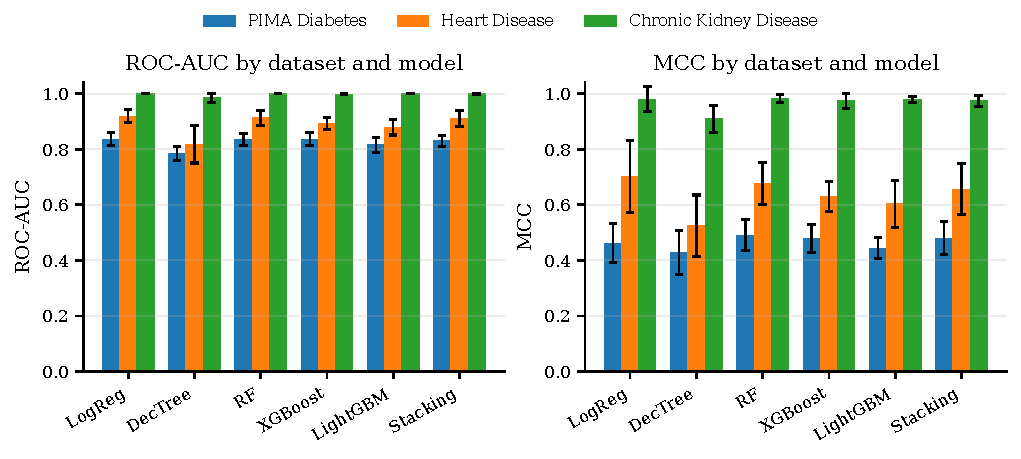
\includegraphics[width=0.88\textwidth]{F3.pdf}\end{center}
\takeaway{ROC-AUC \AucPima{} $\to$ \AucHeart{} $\to$ \AucCkd{}. Chronic Kidney is
near-separable, which turns out to matter for agreement.}
\end{frame}

\begin{frame}{RQ1: SHAP and LIME agree only moderately}
\begin{columns}[T]
\begin{column}{0.58\textwidth}
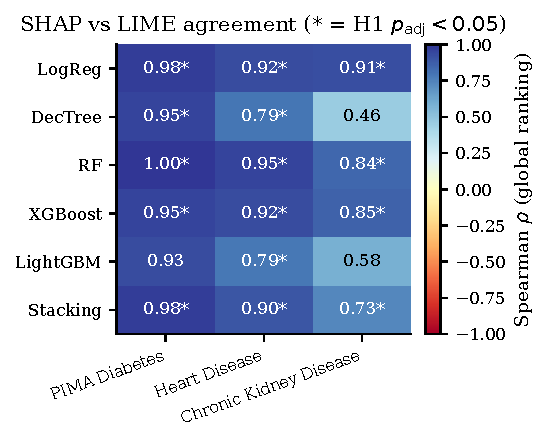
\includegraphics[width=\textwidth]{F4.pdf}
\end{column}
\begin{column}{0.4\textwidth}
\begin{itemize}\setlength\itemsep{0.5em}
  \item Median Spearman $\rho = \MedianRho{}$
  \item Median top-5 Jaccard $= \MedianJaccardFive{}$
  \item Pre-registered bar was $\rho > 0.50$; rejected in \HOneRejected{}/\HOneTotal{}
    cells
\end{itemize}
\end{column}
\end{columns}
\takeaway{On a typical instance the two methods share about half their top five features
and order them differently. Running both is not a robustness check.}
\end{frame}

\begin{frame}{RQ1: agreement does not simply follow task difficulty}
\begin{center}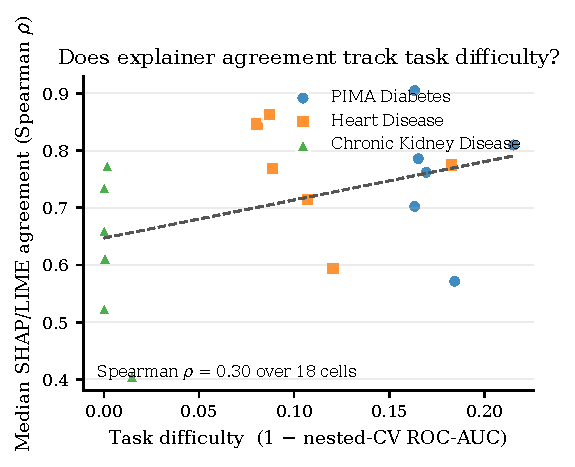
\includegraphics[width=0.62\textwidth]{F6.pdf}\end{center}
\takeaway{Our reading: agreement depends less on difficulty than on feature
\emph{redundancy}. When several features are individually sufficient, both explainers
can be locally faithful while nominating different ones.}
\end{frame}

\begin{frame}{RQ2: reproducible is not the same as robust}
\begin{columns}[T]
\begin{column}{0.5\textwidth}
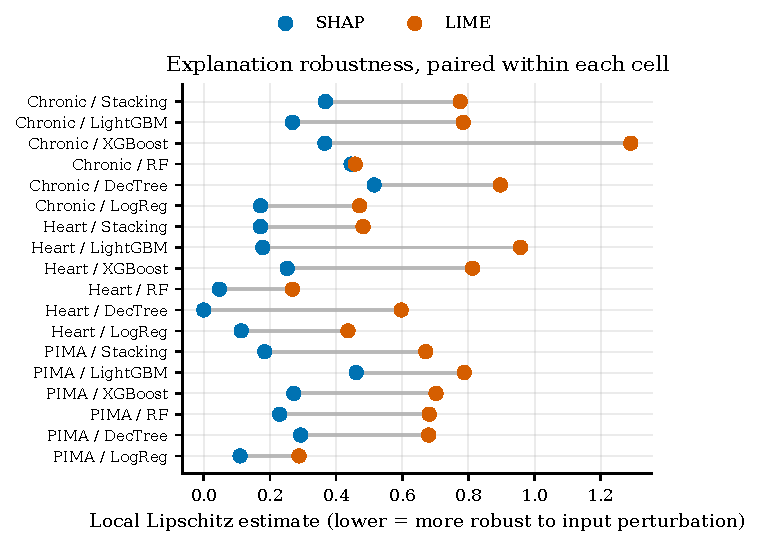
\includegraphics[width=\textwidth]{F8.pdf}
\end{column}
\begin{column}{0.48\textwidth}
\small
\begin{tabular}{@{}lrr@{}}
\toprule
Stability of & \shap{} & \lime{} \\
\midrule
Re-run (CV) & \textbf{0} & \RerunCvLime{} \\
Perturbation ($\hat L$) & \LipschitzShap{} & \LipschitzLime{} \\
Retraining ($\rho$) & \RetrainShap{} & \RetrainLime{} \\
\bottomrule
\end{tabular}
\medskip
\footnotesize Tree \shap{}'s re-run CV is \emph{exactly} zero --- declared a priori in
the protocol, not discovered.
\end{column}
\end{columns}
\takeaway{A perfectly deterministic explanation still moves when the model is refit on a
resample of the same data. That instability is in the model, and determinism cannot fix it.}
\end{frame}

\begin{frame}{RQ3: both are faithful --- and the control is why we can say so}
\begin{center}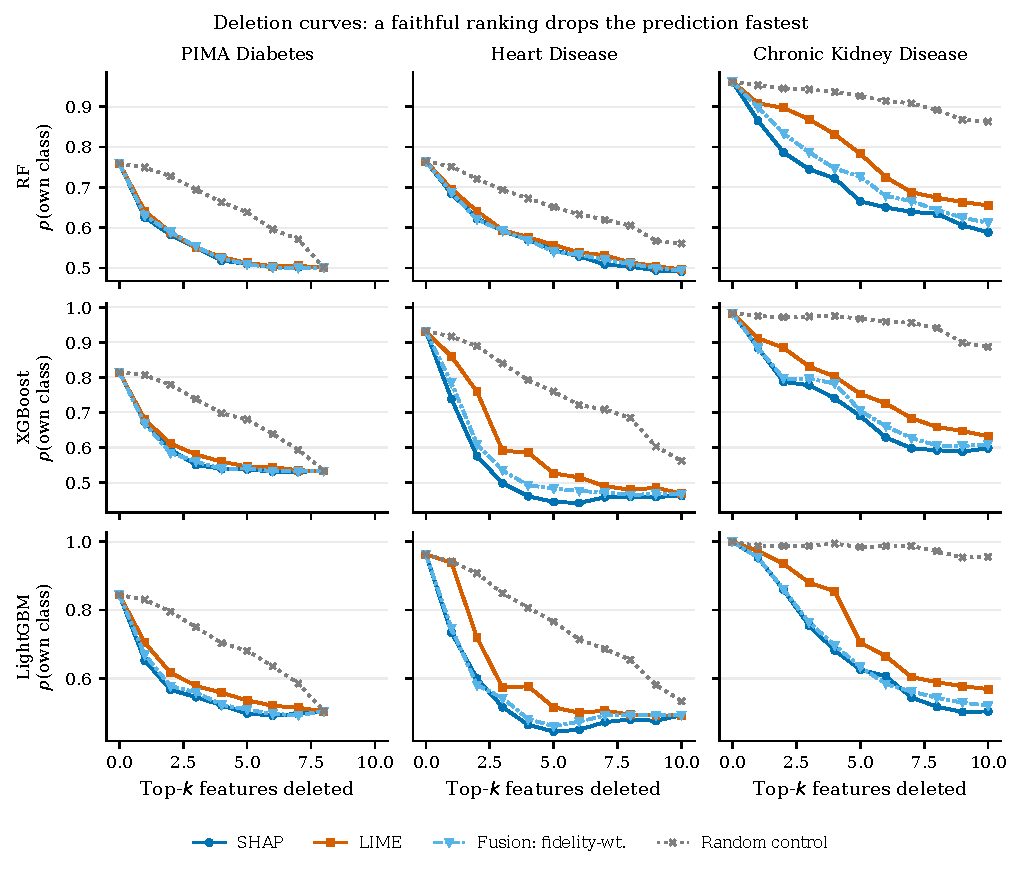
\includegraphics[width=0.82\textwidth]{F10.pdf}\end{center}
\takeaway{\aopc{}: \shap{} \AopcShap{}, \lime{} \AopcLime{}, random \AopcRandom{}.
Beat the control in \HThreeBRejected{}/\HThreeBTotal{} tests after Holm correction.}
\end{frame}

\begin{frame}{RQ4: SHAP is cheaper by roughly an order of magnitude}
\begin{center}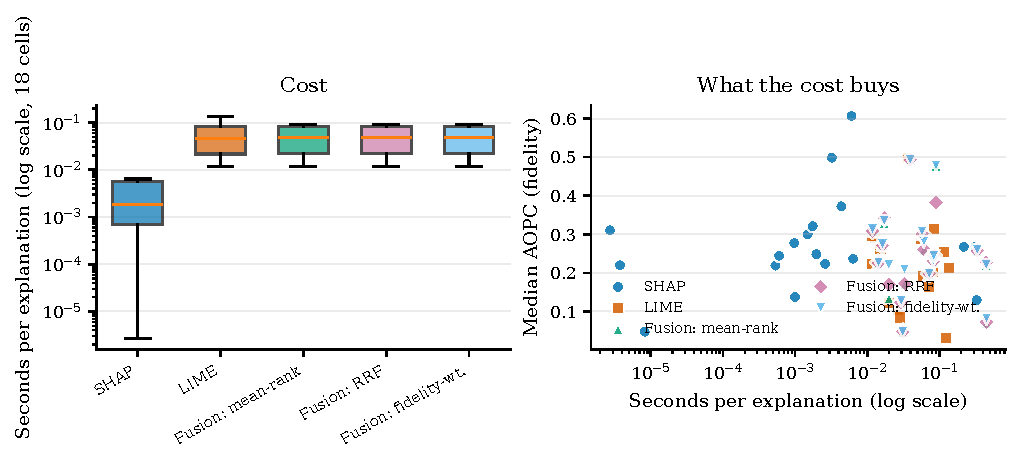
\includegraphics[width=0.9\textwidth]{F11.pdf}\end{center}
\takeaway{\SecondsShap{}\,s versus \SecondsLime{}\,s --- about
\SpeedFactor{}$\times$. Structural, not an implementation detail: \lime{} must evaluate
the model on thousands of perturbed rows per explanation.}
\end{frame}

\begin{frame}{RQ5: the plausibility check does not discriminate --- and we said so first}
\begin{center}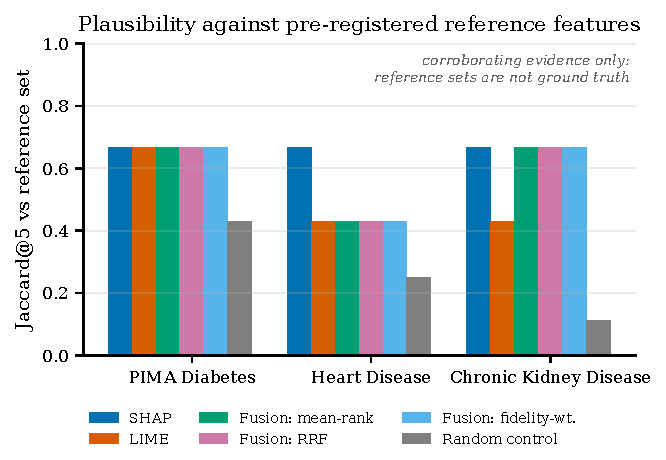
\includegraphics[width=0.68\textwidth]{F12.pdf}\end{center}
\takeaway{Both beat random; neither separates from the other. Literature-derived
reference sets are \emph{not} ground truth, and we pre-registered this as the weakest
measurement in the study.}
\end{frame}

\begin{frame}{RQ6: fusion does not clear the bar --- a pre-registered null result}
\begin{columns}[T]
\begin{column}{0.55\textwidth}
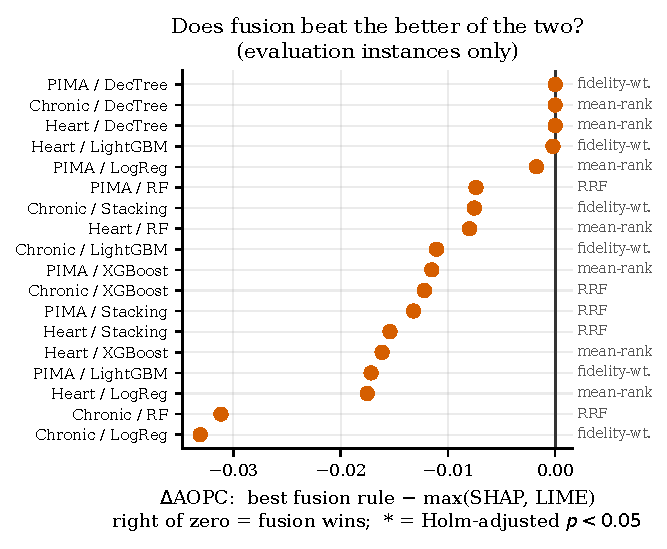
\includegraphics[width=\textwidth]{F13.pdf}
\end{column}
\begin{column}{0.43\textwidth}
\begin{itemize}\setlength\itemsep{0.5em}
  \item Bar: beat the \textbf{better} of the two, not their average
  \item Won in \HSixRejected{} of \HSixTotal{} cells
  \item Best fusion \aopc{} \AopcBestFusion{} vs \shap{} \AopcShap{}
\end{itemize}
\end{column}
\end{columns}
\takeaway{Follows from \RQ{1}: fusion needs \emph{complementary} inputs. Here the two
agree moderately and one is consistently better, so averaging moves toward the weaker.}
\end{frame}

\begin{frame}{All eleven hypotheses, auditable against the frozen protocol}
\begin{center}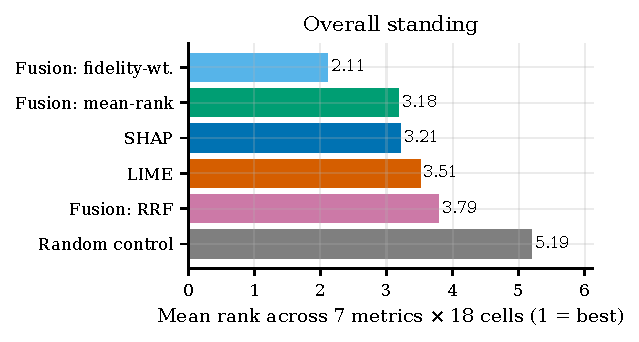
\includegraphics[width=0.62\textwidth]{F14.pdf}\end{center}
\takeaway{The protocol was committed \emph{before} any result existed, so the git
history is itself the evidence that nothing was adjusted after seeing the numbers.}
\end{frame}
